\section{Implementace portace}
\section{Gradle scripts}
Jak bylo popsáno v kapitole \ref{ProposalChapter} jedním z požadavků
\section{Activity and Fragments}

\subsubsection{hard soft score of vrp}

\section{Implementace aplikace}
\section{Material design}
One of the new features which bring Android version 5 is material design. It is very sophisticated study that show how to handle with with elements,
layouts, colors and more. Although this property is not fully backward compatible, it is possible partially to bring this design to earlier devices
with older versions of Android.

This application uses material design as much as possible. Every screen contains material design elements which will be described bellow.

\subsubsection{Components}
\subsubsection{Dialogs}
\subsubsection{Recycler view}
Recycler view


\subsubsection{Application screens}
Every application consists of fragments or activities which are collectively called screens. Using controls, it is
possible to move from one screen to another or change its appearance or behavior. This application is composed from
three screens. These screens can be seen in Figure \ref{screens}. The third screen is displayed with usolved and with
solved solution.

\paragraph{Main screen}
Main screen is displayed after the application is started. It consists from action bar, welcome text, setting elements
and button to continue to another screen. Action bar contains application name and buttons for displaying legend and
application informations dialogs. Two controls are present for calculation options of the problem.

\begin{figure}[h!]
    \centering
    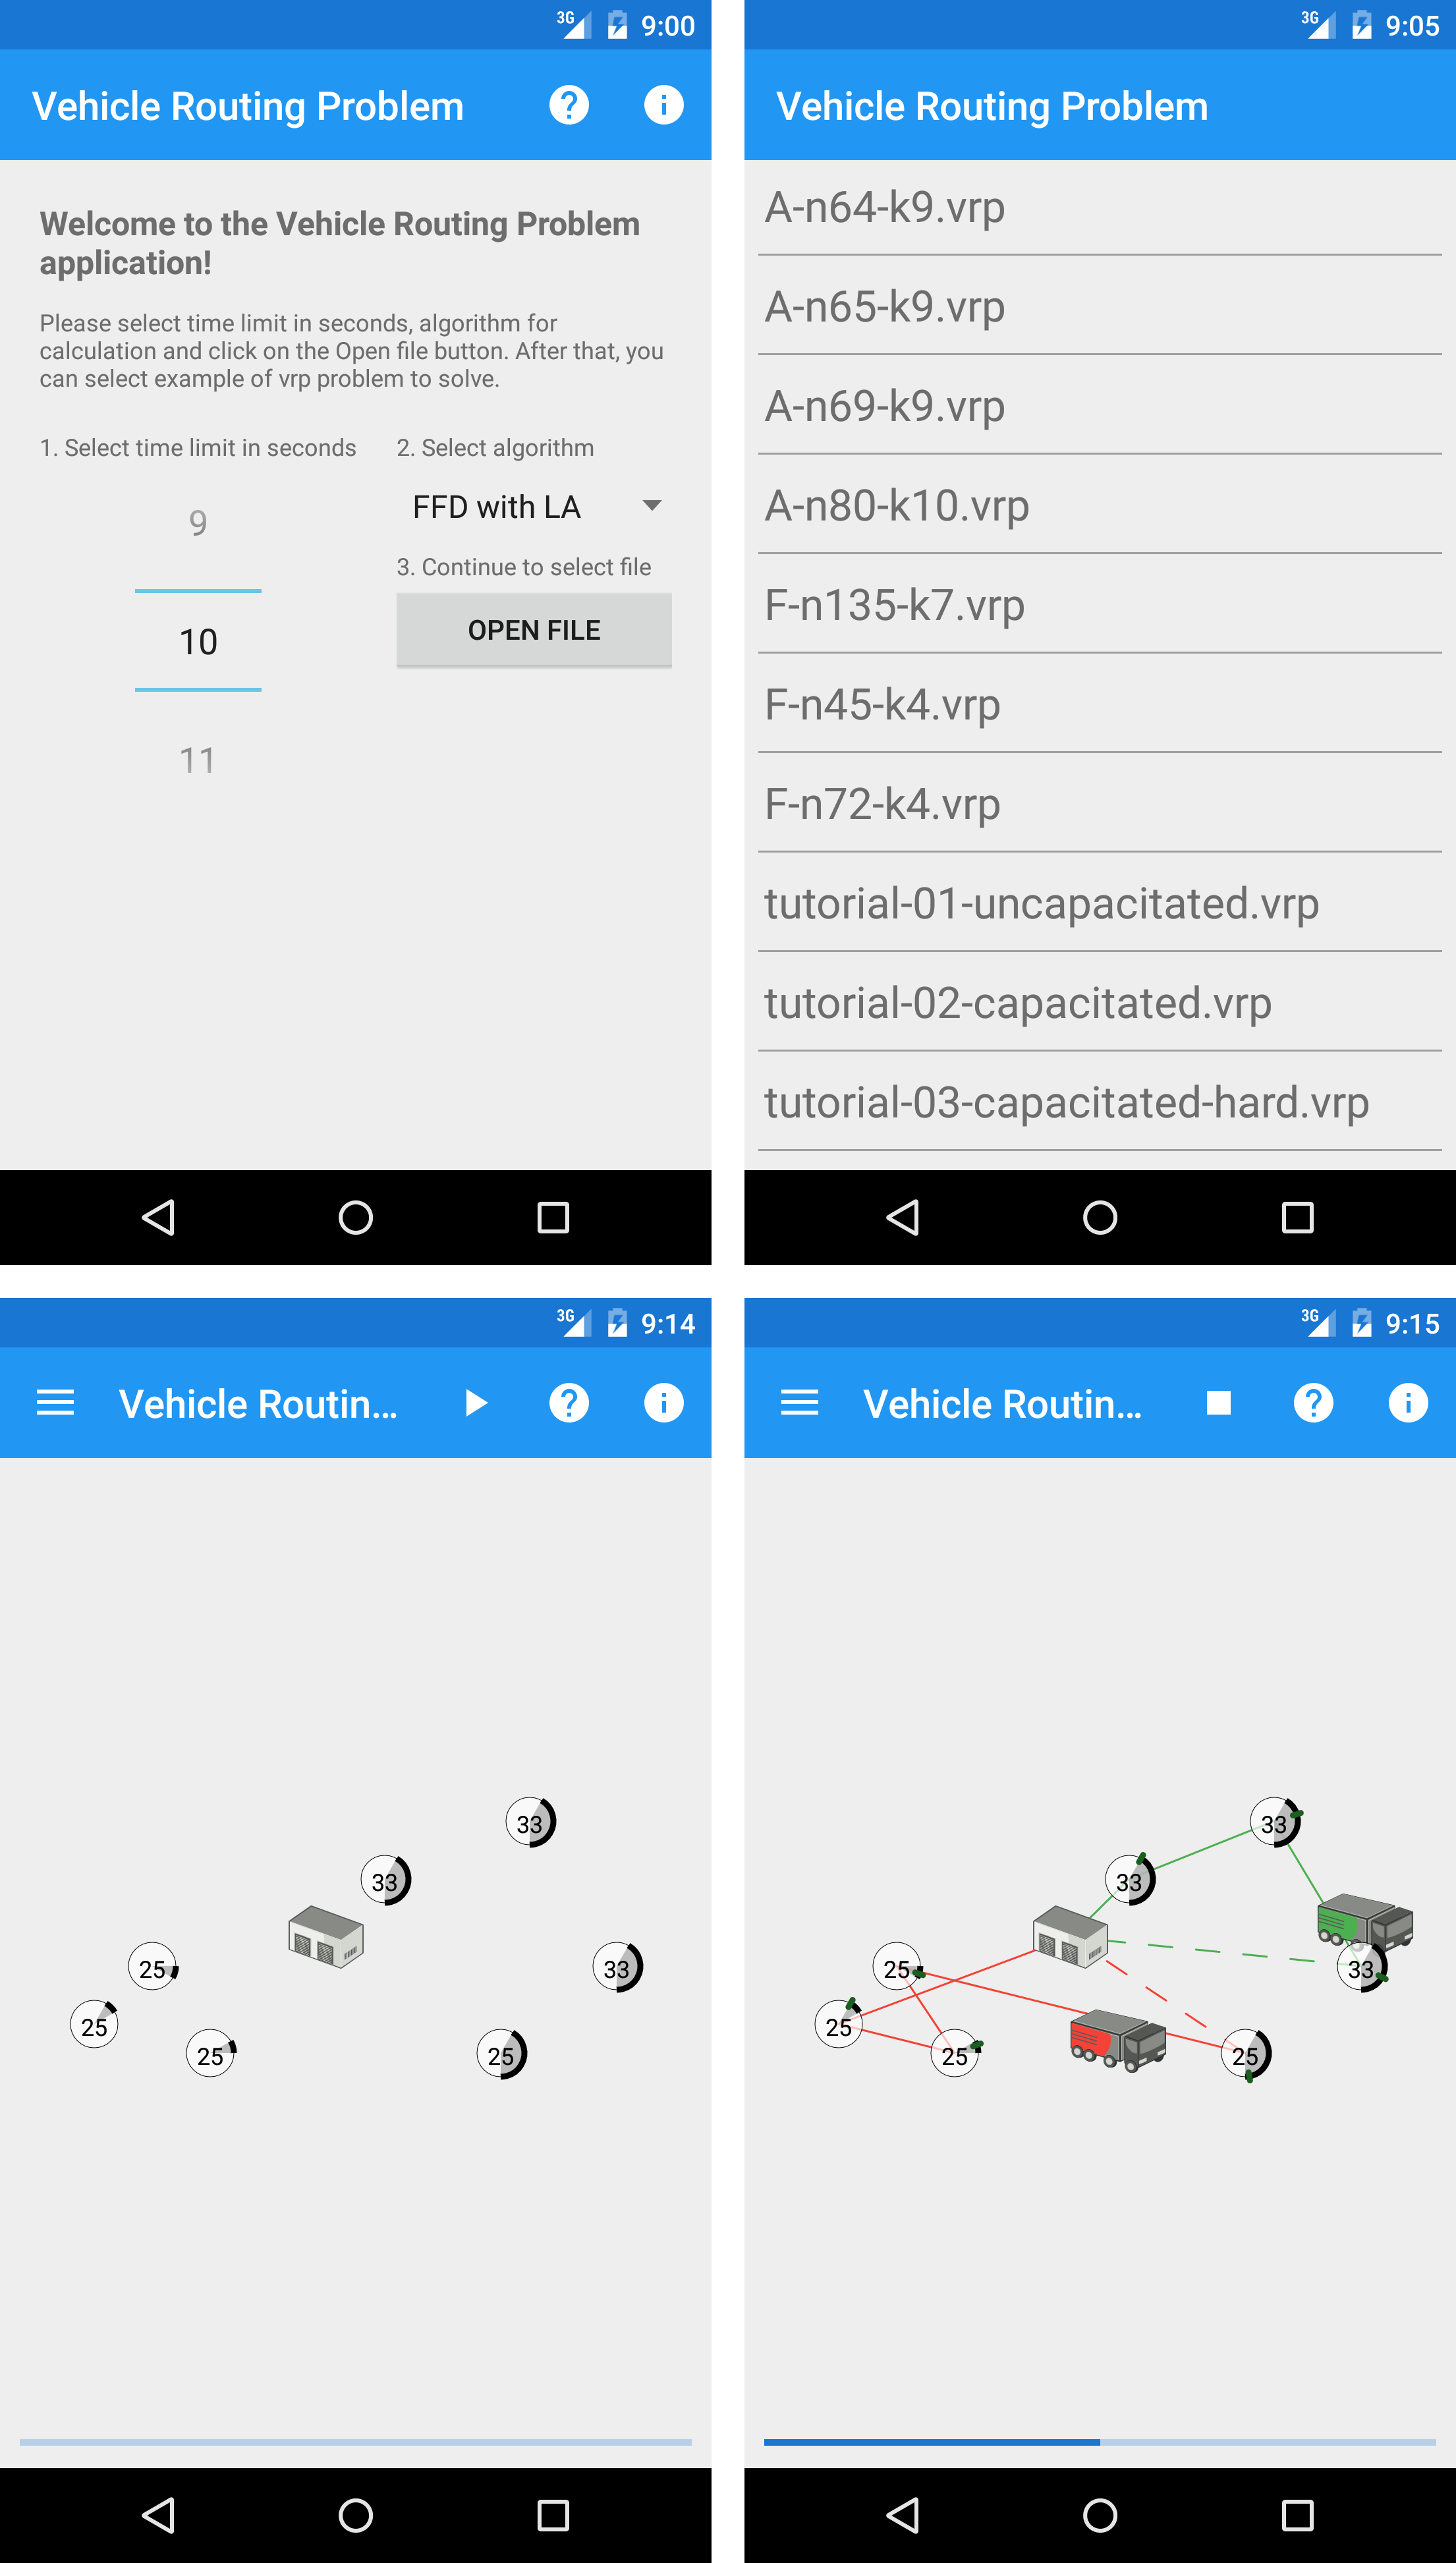
\includegraphics[scale=0.15]{fig/screens.png}
    \caption{Application screens -- main screen, list of vrp files, screen with unsolved and solved solution}
    \label{screens}
\end{figure}

\subsubsection{Action bar}
Action bar is a panel on top of the screen that provides basic user action and informations about user navigation. It
always contains application name, optionally actions buttons for quick invocation of application functionalit and
overflow button on the right side for diplaying other applications options.

Action bar is diplayed on every screen of this application but it changes depending on required functions on actual
screen. Figure \ref{actionBar} show action bar of screen where solved problems are shown. The panel contains buttons for
displaying of navigation drawer and dialogs which are described below and application name.

\begin{figure}[h!]
    \centering
    
\includegraphics[scale=0.15]{fig/action_bar.png}
    \caption{Action bar}
    \label{actionBar}
\end{figure}

\subsubsection{Navigation drawer}
Navigation drawer is a panel that displays application navigation on the left edge of the screen. By default, it is
hidden and it could be displayed by touch the left icon on the action bar. Also it could be displayed whe a user swipes
with a finger from the left edge of the screen to the right. Opposite procedure makes navigation drawer invisible.

This application uses navigation drawer for displaying important computing data. Figure \ref{navigationDrawer} displays
visible panel on the left side of the application. First item shows hard and soft score of currently the best solution
found. Second item holds total distance of all cars. Other items are linked to cars of the problem. Every car has own
parameters -- color, name and capacity. These three are static and do not change during the calculation. Last parametr
is actual load of the vehicle.

\begin{figure}[h!]
    \centering
    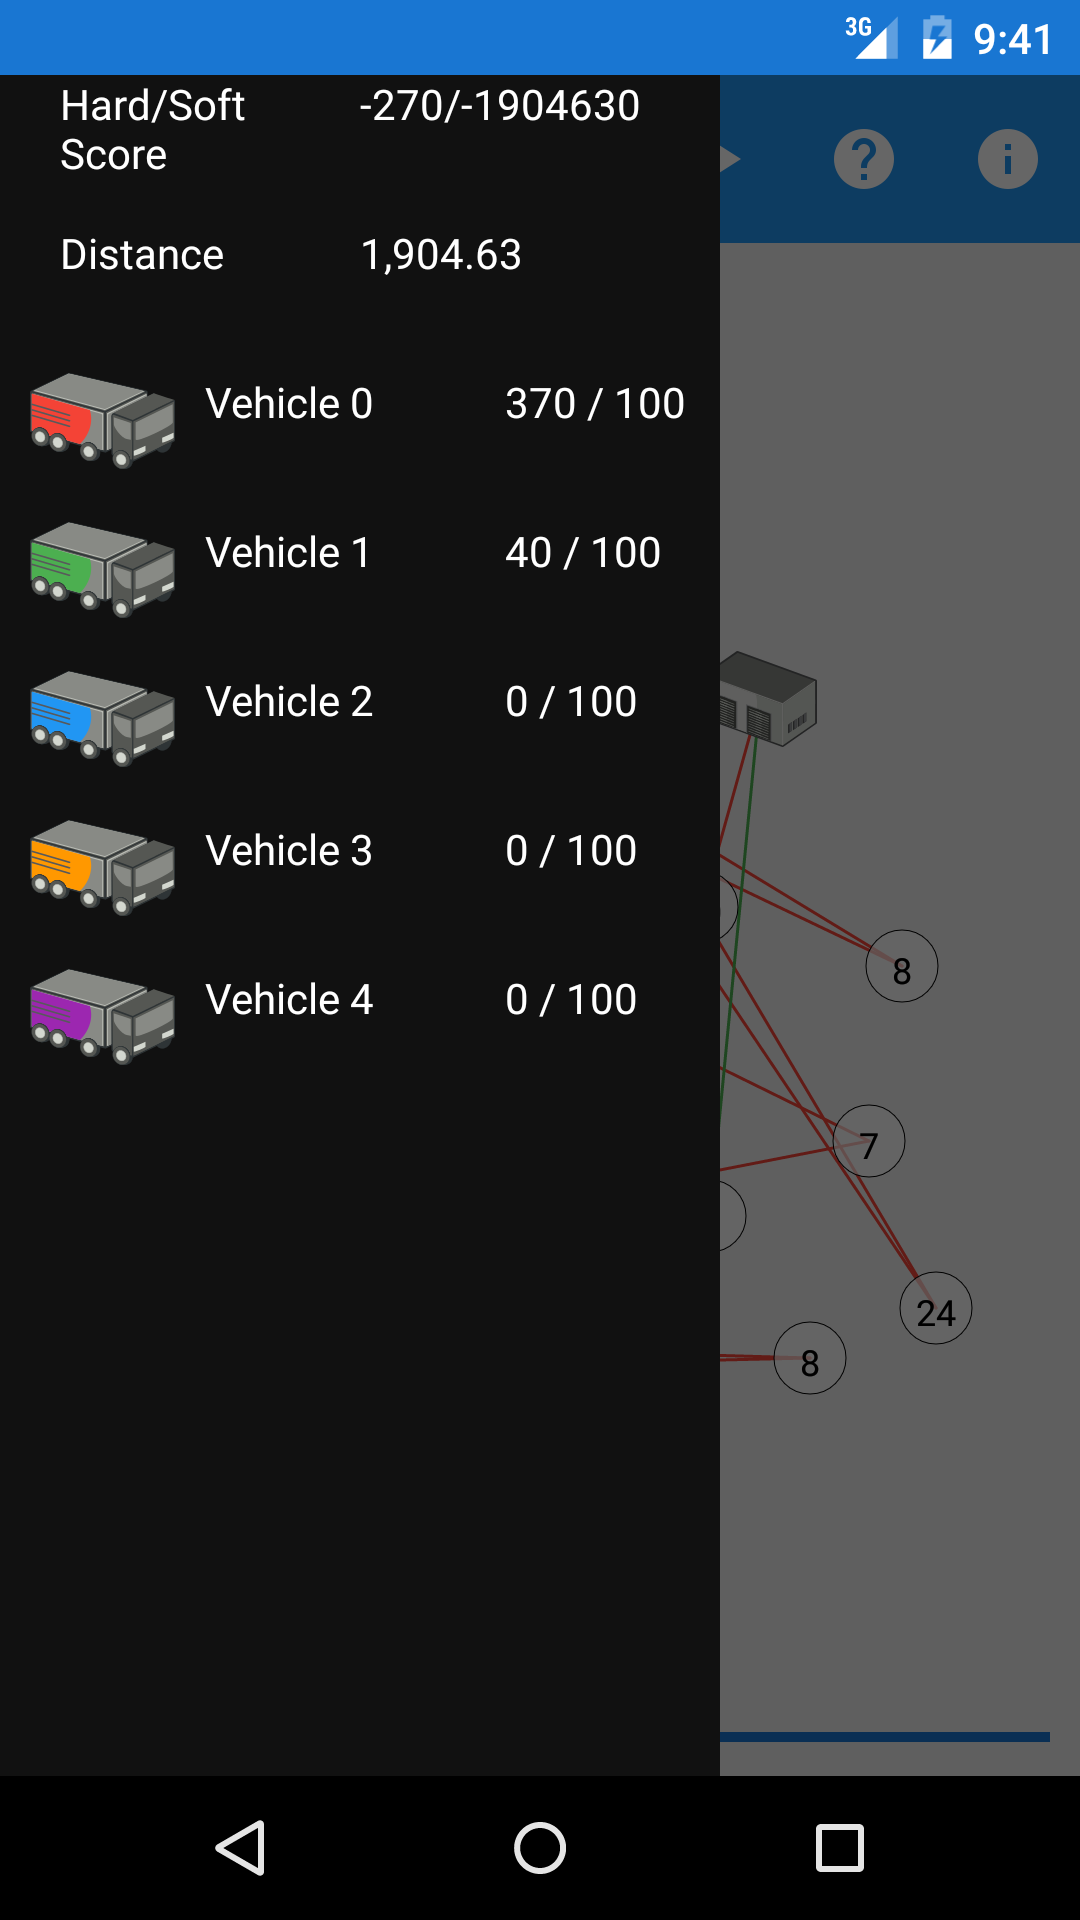
\includegraphics[scale=0.15]{fig/nav_drawer.png}
    \caption{Navigation drawer with actual data}
    \label{navigationDrawer}
\end{figure}

\subsubsection{Dialogs}
Dialogs are small windows which displays some significant informations or are used for user interaction with a decision
that decides on further actions. Dialogs are always located above all other parts of the application

Figure \ref{dialogs} shows all three dialogs which are used in the application. Two of them can be retrieved directly from the
action bar by clicking on the icon with a question mark or the informative icon. First dialog contains application
legend for understanding what is displayed on the screen and second dialog briefly describes the application. Third
dialog is displayed only solving is running and user clicks on the back button. Dialog asks the user if he wants to end
the ongoing calculation.

\begin{figure}[h!]
    \centering
    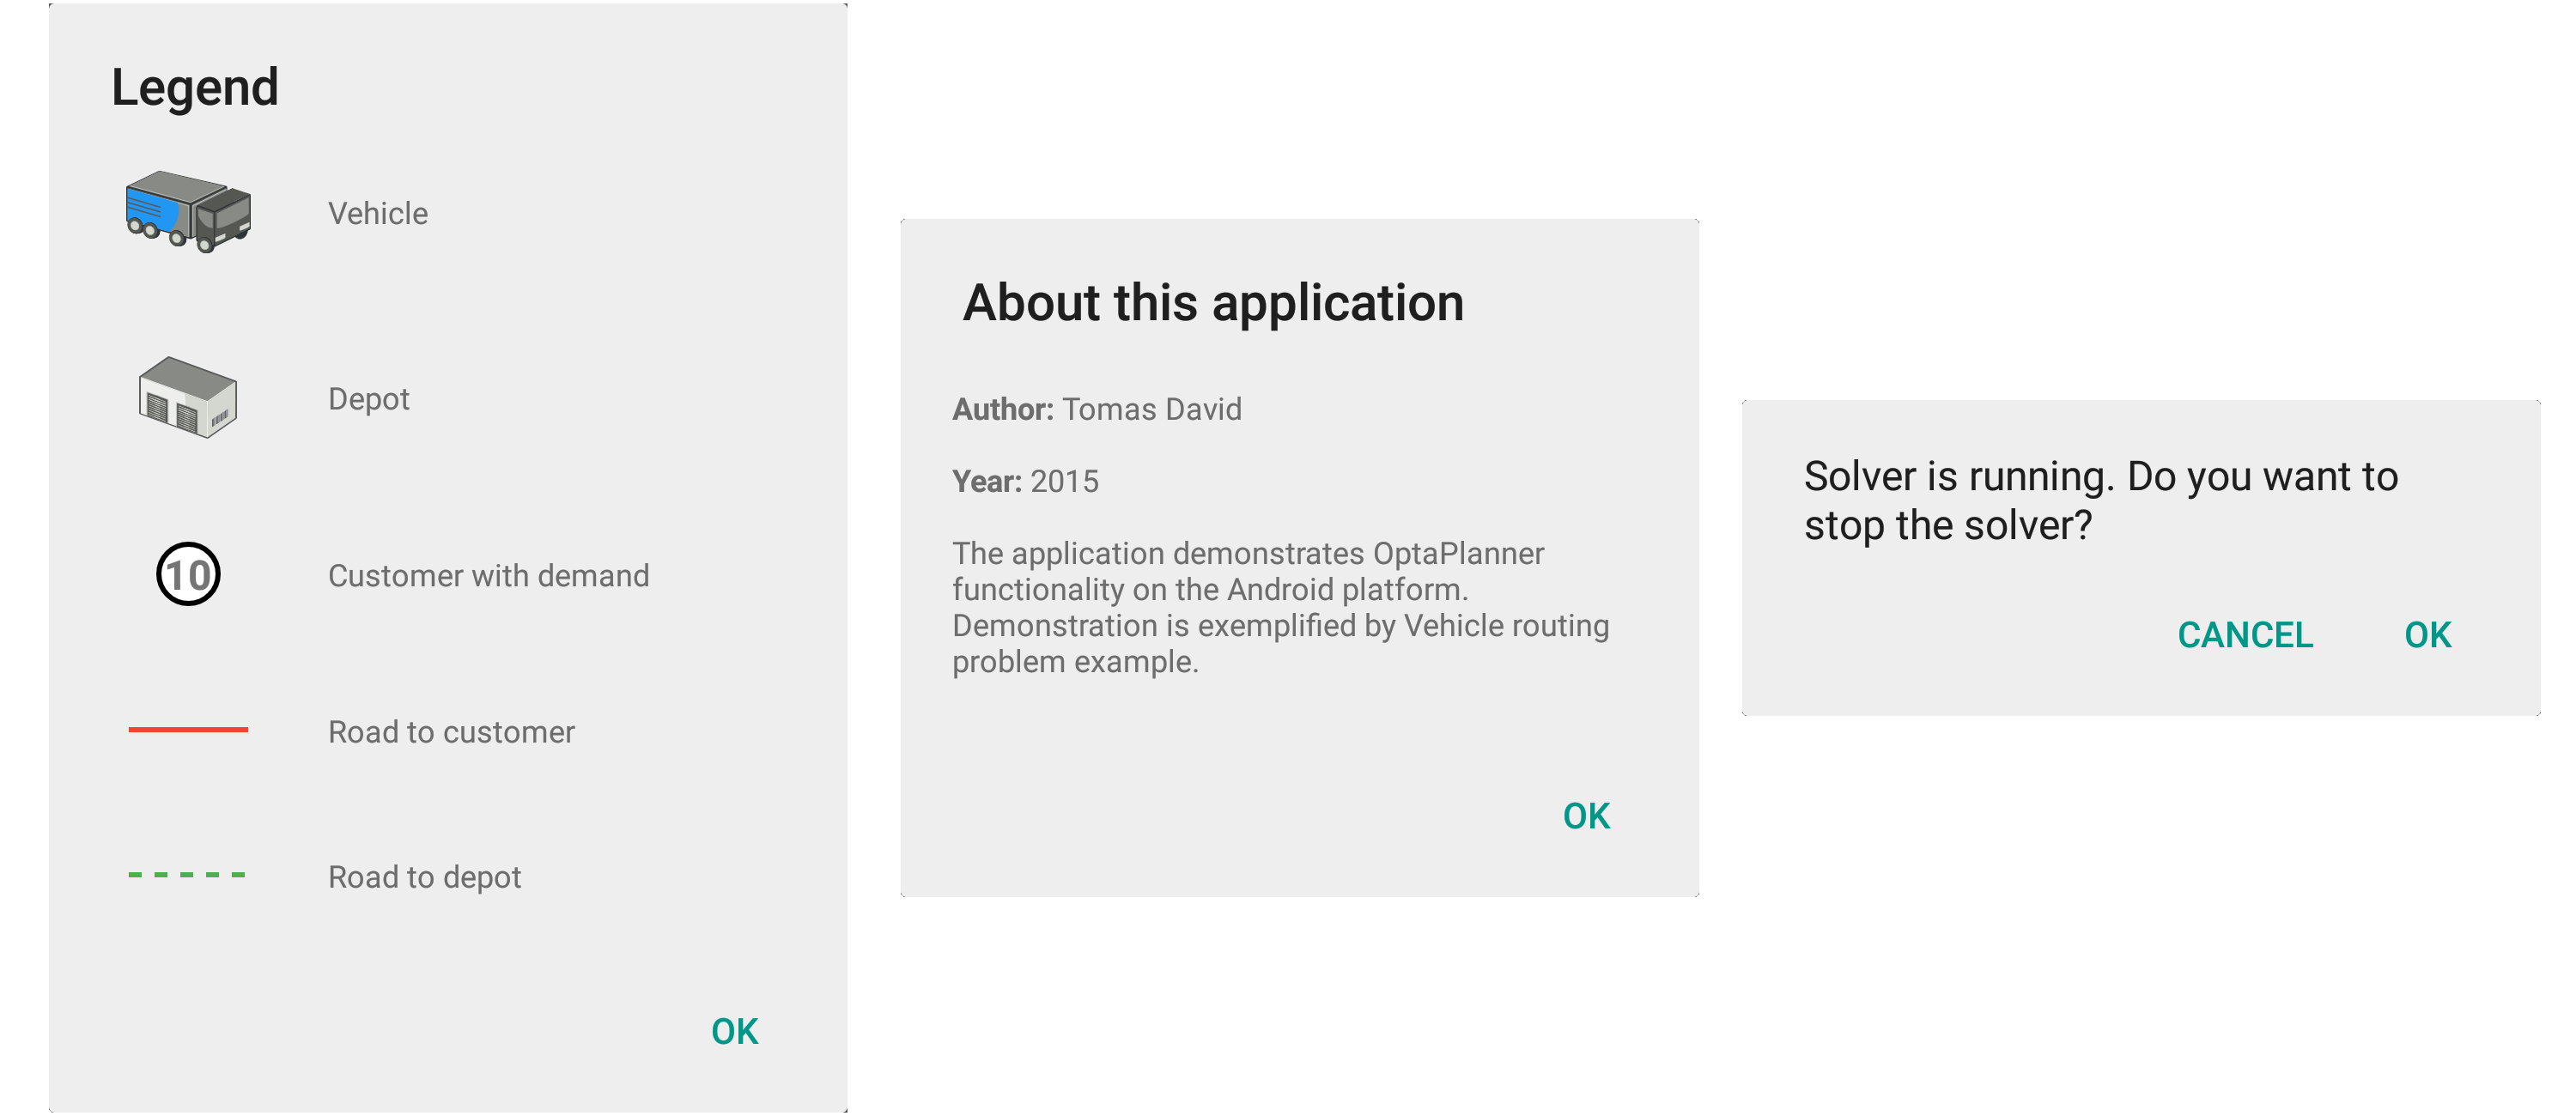
\includegraphics[scale=0.15]{fig/dialogs.png}
    \caption{dialogs used in the application}
    \label{dialogs}
\end{figure}
